\documentclass[a4paper, 12pt]{article}



\usepackage{report}
\usepackage{tabularx}
\usepackage{algorithm}
\usepackage{algpseudocode}
\usepackage{graphicx}
\usepackage{amsmath}
\usepackage{pdfpages}
\usepackage{caption}
\usepackage{amssymb}
\usepackage{listings}
\usepackage[most]{tcolorbox}
\usepackage[table]{xcolor}
\usepackage{multirow}


\usepackage{booktabs}

\renewcommand{\figurename}{Figure~}
\renewcommand{\tablename}{Table~}
\rfoot{Page \thepage\ of \pageref{LastPage}}


% Document Header Setup
\title{\textbf{U2296 Digital System Laboratory}\\ \Large LAB-02: Basic Logic Gates}
\author{Report Template}
\date{}

\begin{document}

\maketitle

\section*{1. Goal}
To verify the operation and characteristics of basic logic gates (NOT, AND, OR).

\section*{2. Theory}
Logic gates and their corresponding truth tables:

\vspace{0.5em}

\noindent
\begin{figure}[htbp]
    \centering
    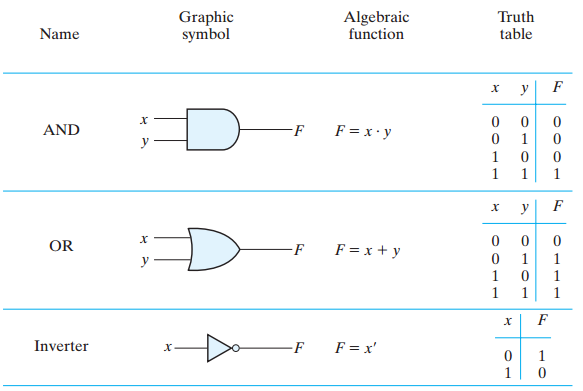
\includegraphics[width=0.8\textwidth]{pic/1.png} % 調整寬度與指定檔名
    \label{fig:fir_image}
\end{figure}

\vspace{1.5em}

\section*{3. Instruments and Components}

\begin{table}[H]
\centering
\small
\begin{tabularx}{0.8\textwidth}{X r}
\toprule
\textbf{Instrument / Component} & \textbf{Quantity} \\
\midrule
DC Power Supply & 1 \\
Breadboard & 1 \\
Multimeter & 1 \\
IC: CD4049 (NOT gate) & 1 \\
IC: CD4081 (AND gate) & 1 \\
IC: CD4071 (OR gate) & 1 \\
LED & 1 \\
Connecting probes and wires & As required \\
\bottomrule
\end{tabularx}
\end{table}

\section*{4. Procedure}
\begin{enumerate}[leftmargin=*]
    \item Place the IC on the breadboard.
    \item Connect IC pin $V_{DD} / V_{CC}$ to $+5\text{V}$ (positive terminal of power supply).
    \item Connect IC pin $V_{SS} / \text{GND}$ to $0\text{V}$ (negative terminal of power supply).
    \item Apply the voltage logic $1$ and logic $0$ separately to \textbf{EACH} input of gates.
    \begin{itemize}
        \item Logic 1 $\rightarrow$ $+5\text{V}$ (positive terminal of power supply)
        \item Logic 0 $\rightarrow$ $0\text{V}$ (negative terminal of power supply)
    \end{itemize}
    \item Connect the outputs to the LED.
    \item Apply various combinations of inputs according to the truth table and observe the status of the LED. Note down the output in the truth table: $1$ (LED ON) and $0$ (LED OFF).
    \item Measure the output voltage using a multimeter. Note down the corresponding multimeter voltage readings for various combinations of inputs in the truth table.
\end{enumerate}

\newpage

\section*{5. Results Summary}
\subsection*{NOT Gate}
\begin{figure}[H] % [H] 強制圖片固定在文字當前的段落位置
    \centering
    % 左邊：圖片區塊
    \begin{minipage}[t]{0.48\textwidth}
        \vspace{0pt} % 修正頂部對齊基準點
        \centering
        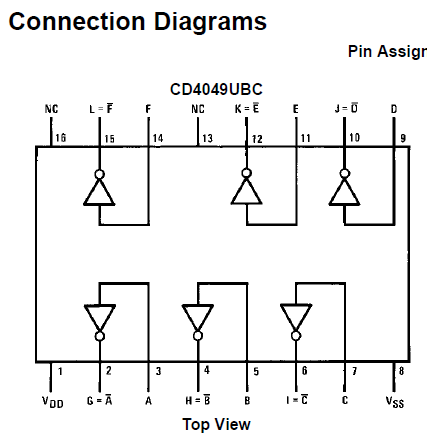
\includegraphics[width=\linewidth]{pic/not gate.png} % 請換成您的圖片檔名
        \captionof{figure}{not gate}
        \label{fig:not_image}
    \end{minipage}
    \hfill % 自動填滿中間間距
    % 右邊：文字區塊
    \begin{minipage}[t]{0.48\textwidth}
        \vspace{0pt} % 修正頂部對齊基準點
        \begin{table}[H]
        \centering
        \begin{tabularx}{0.7\textwidth}{>{\centering\arraybackslash}X | >{\centering\arraybackslash}X | >{\centering\arraybackslash}X}
\toprule
\textbf{Input (A)} & \textbf{O/P (0/1)} & \textbf{O/P (V)} \\
\hline
0 & & \\
1 & & \\
\bottomrule
\end{tabularx}
\end{table}
    \end{minipage}
\end{figure}

\hfill
\subsection*{AND Gate}
\noindent
\begin{figure}[H]
  \centering

   \begin{minipage}[t]{0.48\textwidth}
        \vspace{0pt} % 修正頂部對齊基準點
        \centering
        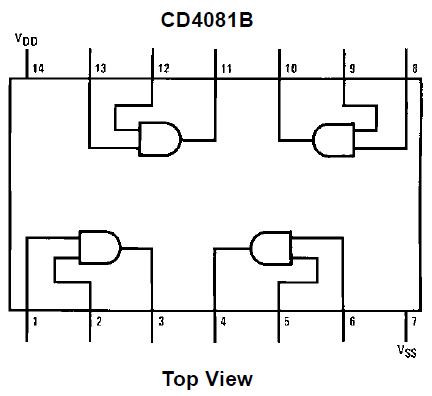
\includegraphics[width=\linewidth]{pic/and gate.png} % 請換成您的圖片檔名
        \captionof{figure}{not gate}
        \label{fig:and_image}
    \end{minipage}
\hfill % 自動填滿中間間距
\begin{minipage}[t]{0.48\textwidth}
  \begin{table}[H]
  \centering
  \small
  \begin{tabularx}{\linewidth}{c c | >{\centering\arraybackslash}X | >{\centering\arraybackslash}X}
  \toprule
  \textbf{In A} & \textbf{In B} & \textbf{O/P (0/1)} & \textbf{O/P (V)} \\
  \hline
  0 & 0 & & \\
  0 & 1 & & \\
  1 & 0 & & \\
  1 & 1 & & \\
  \bottomrule
  \end{tabularx}
  \end{table}
\end{minipage}
\end{figure}
\hfill

\subsection*{AND Gate}
\noindent
\begin{figure}[H]
  \centering

   \begin{minipage}[t]{0.48\textwidth}
        \vspace{0pt} % 修正頂部對齊基準點
        \centering
        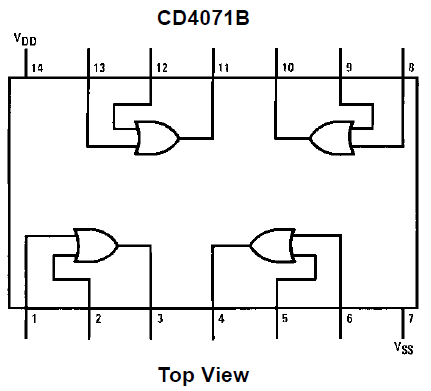
\includegraphics[width=\linewidth]{pic/or gate.png} % 請換成您的圖片檔名
        \captionof{figure}{not gate}
        \label{fig:or_image}
    \end{minipage}
\begin{minipage}[t]{0.48\textwidth}
  \begin{table}[H]
  \centering
  \small
  \begin{tabularx}{\linewidth}{c c | >{\centering\arraybackslash}X | >{\centering\arraybackslash}X}
  \toprule
  \textbf{In A} & \textbf{In B} & \textbf{O/P (0/1)} & \textbf{O/P (V)} \\
  \hline
  0 & 0 & & \\
  0 & 1 & & \\
  1 & 0 & & \\
  1 & 1 & & \\
  \bottomrule
  \end{tabularx}
  \end{table}
\end{minipage}
\end{figure}

\vspace{1.5em}

\section*{6. Problems and Discussion}
Discuss any problems encountered during the procedure.








\vspace{5cm}

\section*{Student Feedback (Lab-02)}
\textit{The last part of the lab requests your feedback. We are continually trying to improve the laboratory exercises to enhance your learning experience, and we are unable to do so without your feedback. Please include the following post-lab deliverables in your lab write-up.}

\begin{enumerate}[leftmargin=*]
    \item What did you like most about the lab assignment and why?
    \item What did you like least about it and why?
    \item Was there any section of the lab handout that was unclear? If so, what was unclear? Do you have any suggestions for improving the clarity?
    \item What suggestions do you have to improve the overall lab assignment?
\end{enumerate}

\end{document}